

\chapter{Contact}

\section{Implicit Contact Solver}

The contact formulation corresponds to the augmented-Lagrangian method \cite{Laursen:2002}, which seeks to minimize the following energy functional between two bodies with contact interface $ \Gamma_c^{\left( 1 \right)} $:
\begin{equation} \label{eq:functinal}
  \Pi^{al} \left( \boldsymbol u, \lambda_N \right) := \sum_{i=1}^2 \Pi ^{\left( i \right) } ( \boldsymbol u ^{\left( i \right) }  ) + \int_{\Gamma_c^{\left( 1 \right) } } \left[ \frac{1}{2 \epsilon_N } \left< \lambda_N + \epsilon_N g \right>^ 2 - \frac{1}{2 \epsilon_N} \lambda^2_N \right] \, d\Gamma,
\end{equation}
where $ \Pi^{\left( i \right) } $ corresponds to the energy functional of the $ i $-th body in contact, which is a function of the displacement field $\boldsymbol u$ and the Lagrangian multiplier $\lambda_N$. In the equation above, $\epsilon_N$ is a penalty parameter,  $g$ the contact gap function, and $\left< \cdot \right>$ the Macaulay bracket.

The solution procedure seeks to make the equation above stationary with respect to both $\boldsymbol u$ and $\lambda_N$:
\begin{equation}
\begin{aligned}
 0 &= D_{\boldsymbol u} \Pi^{al} \cdot \boldsymbol w = G^{int,ext} \left( \boldsymbol u, \boldsymbol w \right) + \int_{\Gamma_c^{\left( 1 \right) } } \left< \lambda_N + \epsilon_N g \right> \delta g  \, d\Gamma  \qquad  \forall \boldsymbol w \in \mathcal{V} \\
0 &= D_{ \lambda} \Pi^{al} \cdot q_N  = \frac{1}{\epsilon_N} \int_{\Gamma_c^{\left( 1 \right) } } \left[ \left< \lambda_N + \epsilon_N g \right> - \lambda_N \right] q_N  \, d\Gamma  \qquad  \forall q_N \in \mathcal{M}
\end{aligned}
\end{equation}

A solution is then found by using Uzawa's method, for which we solve for $ \boldsymbol u ^ {\left( k \right) }$, with $ \lambda_N^{\left( k \right)}$ fixed:
\begin{equation}
 G^{int,ext} ( \boldsymbol u ^ {\left( k \right) }, \boldsymbol w ) + \int_{\Gamma_c^{\left( 1 \right) } } \left< \lambda_N^ {\left( k \right) } + \epsilon_N g( \boldsymbol u ^ {\left( k \right) } )  \right> \delta g  \, d\Gamma = 0 \qquad \forall \boldsymbol w \in \mathcal{V},
 \end{equation}

followed by an update of the multipliers on $\Gamma_c ^ {\left( 1 \right) }$:
\begin{equation}
\lambda _N ^ {\left( k+1 \right) } = \left< \lambda_N ^ {\left( k \right) } + \epsilon_N g ( \boldsymbol u ^ {\left( k \right) } ) \right>.
\end{equation}


It is worth noting that the results of the implicit contact resolution depend largely on the choice of the penalty parameter $ \epsilon_N $. Depending on this parameter, the computational time needed to obtain a converged solution can be increased dramatically, or a convergence solution could not even be obtained at all.

The code provides a flag that allows the user to rely on an automatic value of $ \epsilon_N $ for each slave node. Yet, this value should be used as a reference only, since for some problems it is actually overestimated and convergence cannot be obtained.


\subsection{Implementation}

In \akantu, the object that handles the implicit contact can be found in \code{implicit\_contact\_manager.hh}.
The object that handles the implicit contact resolution stage is the class template
\begin{cpp}
template <int dim, class model_type> struct ContactData;
\end{cpp}
This object takes the command line parameters during construction, which can be used to set up the behavior during contact resolution. The object can take the following parameters (default values in brackets):

\begin{tabular}{lrl}
  -e & [auto] & Penalty parameter for augmented-Lagrangian formulation \\
  -alpha & [1] & Multiplier for values of the penalty parameter\\
 -utol & [0.001] & Tolerance used for multipliers in the Uzawa method\\
 -ntol &[0.001]& Tolerance used in the Newton-Raphson inner convergence loop\\
 -usteps &[100]&  Maximum number of steps allowed in the Uzawa loop\\
 -nsteps & [100]&  Maximum number of steps allowed in the Newton-Raphson loop\\
\end{tabular} \\


Also, the following flags can be given to the command line


\begin{tabular}{ll}
 -dump&          Dumping within Newton iterations \\
 -v&             Verbose output
\end{tabular} \\



The \code{ContactData} object stores the state of the contact mechanics simulation. The state is contained within the following variables:

\begin{tabular}{ll}
 \code{sm\_}  & slave-master map \\
 \code{multipliers\_} & Lagrange multiplier map \\
 \code{areas\_} & slave areas map \\
 \code{penalty\_} & penalty parameter map \\
 \code{gaps\_} & gap function map \\
 \code{model\_} & reference to solid mechanics model \\
 \code{multiplier\_dumper\_} & structures used to dump multipliers \\
  \code{pressure\_dumper\_} & structures used to dump pressure \\
 \code{options\_} & options map \\
 \code{flags\_} & flags map \\
 \code{uiter\_}, \code{niter\_} & Uzawa and Newton iteration counters
\end{tabular} \\


The interface of the \code{ContactData} object contains three methods to solve for each contact step, which is overloaded depending on the parameters passed. Their signatures are as follows


\begin{cpp}
void solveContactStep();

void solveContactStep(search_type *search);

template <class PostAssemblyFunctor>
void solveContactStep(search_type *search, const PostAssemblyFunctor& fn);
}
\end{cpp}

The second method allows the user to provide a pointer to an object that is used to search slave-master pairs. This can be done, for example, when due to the deformed configuration current slave-master pairs are no longer valid.
The last method in the snippet above allows the user to provide a functor that is called after the assembly of the contact contributions to the stiffness matrix and the force vector. The last takes place within the method \code{computeTangentAndResidual()}.


\subsubsection{Hertz Example}


Here we outline, step by step, the use of the implicit contact solver to obtain the solution of Hertzian contact. The complete implementation can be found in \code{examples/contact/hertz\_3D.cc}.

The following class is used as the object that will perform the search for new contact elements when a slave node is found to lie outside its master element. The class derives from a \code{SearchBase} class, and implements the virtual method \code{search}.

\begin{cpp}
struct Assignator : public ContactData<3,SolidMechanicsModel>::SearchBase {
  typedef Point <3> point_type;
  typedef SolidMechanicsModel model_type;
  typedef ModelElement <model_type> master_type;

  model_type &model_;

  Assignator(model_type& model) : model_(model) {}

  virtual int search(const Real *ptr) {
    point_type p(ptr);

    ElementGroup &rs = model_.getMesh().getElementGroup("rigid_surface");

    for (ElementGroup::type_iterator tit = rs.firstType(); tit != rs.lastType(); ++tit)
      for (ElementGroup::const_element_iterator it = rs.element_begin(*tit);
           it != rs.element_end(*tit); ++it) {
        master_type m(model_, _triangle_3, *it);
        if (point_has_projection_to_triangle(p, m.point <3>(0), m.point <3>(1), m.point <3>(2))) {
          return m.element;
        }
      }
    return -1;
  }
};
\end{cpp}


The first thing we do in the main file is to add some type definitions:

\begin{cpp}

int main(int argc, char *argv[]) {

  // set dimension
  static const UInt dim = 3;

  // type definitions
  typedef Point <dim> point_type;
  typedef BoundingBox <dim> bbox_type;
  typedef SolidMechanicsModel model_type;
  typedef ModelElement <model_type> master_type;
  typedef ContactData <dim, model_type> contact_type;

  typedef std::chrono::high_resolution_clock clock;
  typedef std::chrono::seconds seconds;
\end{cpp}

We initialize the library, create a mesh, and set the solid mechanics model up:

\begin{cpp}

  initialize("steel.dat", argc, argv);

  // create mesh
  Mesh mesh(dim);

  // read mesh
  mesh.read("hertz_3D.msh");

  // create model
  model_type model(mesh);
  SolidMechanicsModelOptions opt(_static);

  // initialize material
  model.initFull(opt);
\end{cpp}


Then we create the contact data, which can be used to solve the contact problem. Note that some of the parameters required by the contact object can be coded in the implementation file (these can also be passed as arguments).
\begin{cpp}

  // create data structure that holds contact data
  contact_type cd(argc, argv, model);

  // optimal value of penalty multiplier
  cd[Alpha] = 0.05;
  cd[Uzawa_tol] = 1.e-2;
  cd[Newton_tol] = 1.e-2;
\end{cpp}


Next we find the area that corresponds to each slave node. For this we use the fact that if we apply a unit distributed load over the contact surface, the resulting force vector at each slave node has magnitude that is equal to the area.
\begin{cpp}

  // get physical names from Gmsh file
  mesh.createGroupsFromMeshData <std::string>("physical_names");

  // get areas for the nodes of the circle
  // this is done by applying a unit pressure to the contact surface elements
  model.applyBC(BC::Neumann::FromHigherDim(Matrix <Real>::eye(3, 1.)), "contact_surface");
  Array <Real>& areas = model.getForce();

  // loop over contact surface nodes and store node areas
  ElementGroup &eg = mesh.getElementGroup("contact_surface");
  cout << "- Adding areas to slave nodes. " << endl;
  for (auto nit = eg.node_begin(); nit != eg.node_end(); ++nit) {
    // compute area contributing to the slave node
    Real a = 0.;
    for (UInt i = 0; i < dim; ++i)
      a += pow(areas(*nit, i), 2.);
    cd.addArea(*nit, sqrt(a));
  }

  // set force value to zero
  areas.clear();
\end{cpp}

Note that we clear the force vector after the assignment of areas.

In the next step we prescribe the boundary conditions that do not change in time:

\begin{cpp}

  // apply boundary conditions for the rigid plane
  model.applyBC(BC::Dirichlet::FixedValue(0., BC::_x), "bottom_body");
  model.applyBC(BC::Dirichlet::FixedValue(0., BC::_y), "bottom_body");
  model.applyBC(BC::Dirichlet::FixedValue(0., BC::_z), "bottom_body");

  // block z-disp in extreme points of top surface
  model.getBoundary()(1, 2) = true;
  model.getBoundary()(2, 2) = true;

  // block x-disp in extreme points of top surface
  model.getBoundary()(3, 0) = true;
  model.getBoundary()(4, 0) = true;

\end{cpp}


Next we add the slave-master pairs for the analysis. We use a bounding box to consider only a fraction of the slave nodes in the model. Those slave nodes that are not within the bounding box are not considered in the analysis:
\begin{cpp}

  // set-up bounding box to include slave nodes that lie inside it
  Real l1 = 1.;
  Real l2 = 0.2;
  Real l3 = 1.;
  point_type c1(-l1 / 2, -l2 / 2, -l3 / 2);
  point_type c2(l1 / 2,  l2 / 2,  l3 / 2);
  bbox_type bb(c1, c2);

  // search policy for slave-master pairs
  Assignator a(model);


  // loop over nodes in contact surface to create contact elements
  cout << "- Adding slave-master pairs" << endl;
  for (auto nit = cs.node_begin(); nit != cs.node_end(); ++nit) {
    point_type p(&coords(*nit));

    // ignore slave node if it doesn't lie within the bounding box
    if (!(bb & p))
      continue;

    int el = a.search(&coords(*nit));
    if (el != -1)
      cd.addPair(*nit, master_type(model, _triangle_3, el));
  }
\end{cpp}


We then start the loop over displacement increments, and at each step we call {{{solveContactStep}}} and save the displacement, resulting force, and maximum pressure, in an array that will be used to print the results at the end of the simulation:
\begin{cpp}

  const size_t steps = 30;
  Real data[3][steps]; // store results for printing
  Real step = 0.001;  // top displacement increment
  size_t k = 0;

  for (Real delta = 0; delta <= step * steps; delta += step) {
    // apply displacement to the top surface of the half-sphere
    model.applyBC(BC::Dirichlet::FixedValue(-delta, BC::_y), "top_surface");

    // solve contact step, this method also dumps Paraview files
    cd.solveContactStep(&a);

    data[0][k] = delta;
    data[1][k] = cd.getForce();
    data[2][k] = cd.getMaxPressure();
    ++k;
  }
\end{cpp}


The last portion of the output of code above is as follows:
\begin{verbatim}
         Disp.         Force  Max pressure
             0             0             0
         0.001          1.29     6.068e+04
         0.002     6.702e+06      6.78e+09
         0.003     1.832e+07     9.453e+09
         0.004     3.349e+07     1.091e+10
         0.005       5.2e+07     1.171e+10
         0.006     7.211e+07     1.298e+10
         0.007     9.377e+07     1.481e+10
         0.008     1.183e+08     1.624e+10
         0.009      1.41e+08     1.616e+10
          0.01       1.7e+08     1.688e+10
         0.011     1.963e+08     1.678e+10
         0.012     2.263e+08     1.758e+10
         0.013     2.581e+08     1.805e+10
         0.014     2.907e+08     1.821e+10
         0.015     3.244e+08     1.877e+10
         0.016     3.593e+08     1.954e+10
         0.017     4.051e+08     2.131e+10
         0.018     4.317e+08     2.115e+10
         0.019     4.823e+08     2.201e+10
          0.02     5.237e+08     2.315e+10
         0.021     5.639e+08     2.379e+10
         0.022     6.058e+08     2.405e+10
         0.023     6.483e+08     2.485e+10
         0.024     6.917e+08     2.536e+10
         0.025     7.363e+08     2.854e+10
         0.026     7.681e+08     3.099e+10
         0.027     8.332e+08     3.291e+10
         0.028     8.577e+08     3.399e+10
         0.029     9.281e+08     3.426e+10
\end{verbatim}

The following figure shows the deformed state of the half-sphere at the end of the simulation, together with the contact pressure distribution:

\begin{figure}[htbp]
\begin{center}
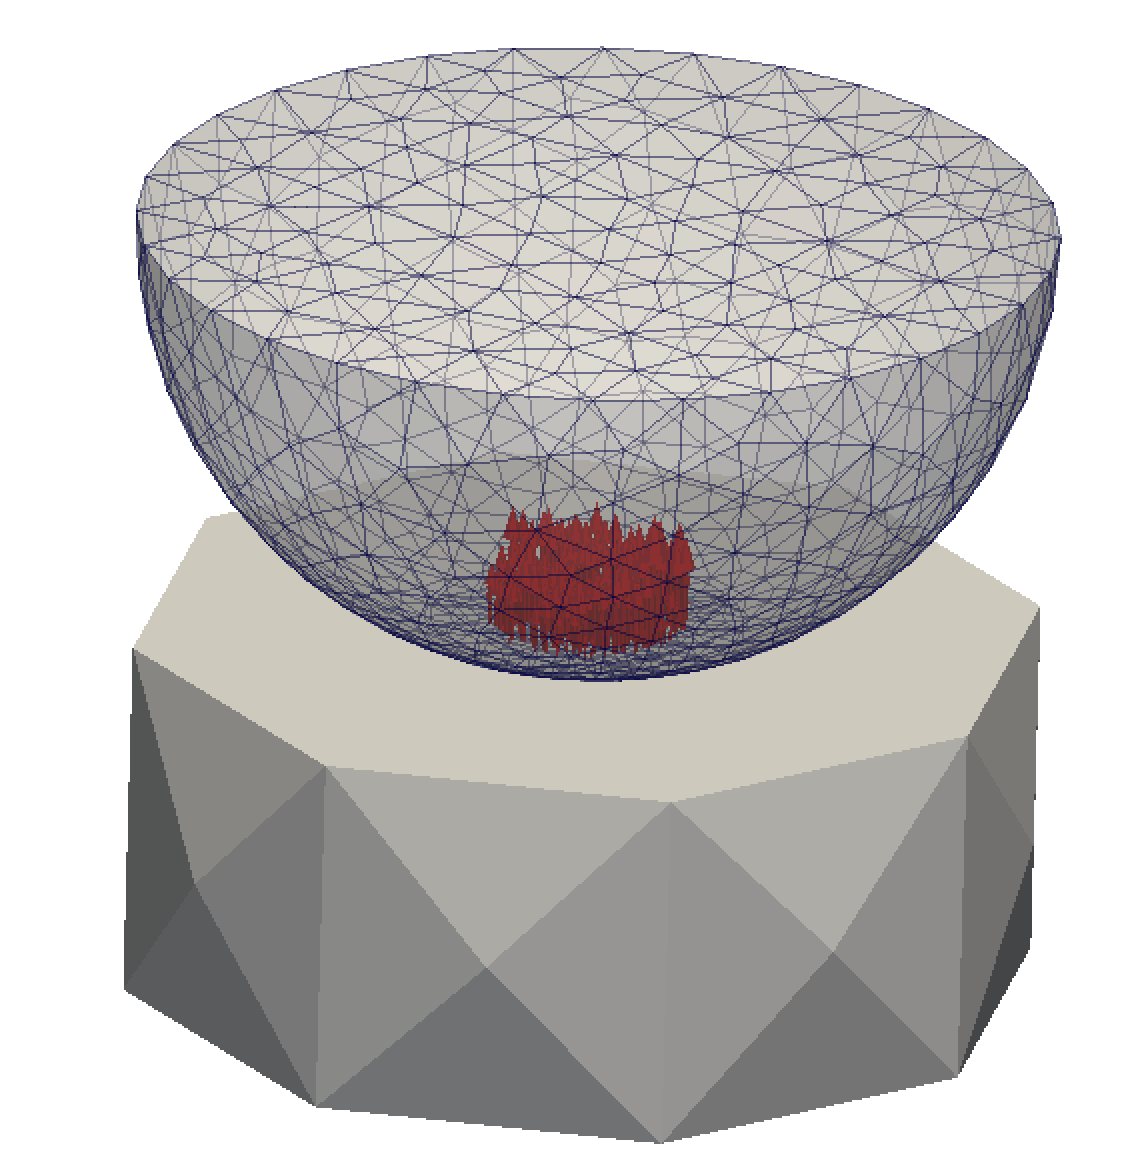
\includegraphics[scale=0.3]{figures/hertz_3D.png}
\caption{State of pressure and deformation at the end of the simulation of the example of Hertz in 3D.}
\label{fig:hertz_3D}
\end{center}
\end{figure}
